\documentclass{beamer}
\usepackage[utf8]{inputenc}
\usetheme{Copenhagen}

\usepackage[export]{adjustbox}

\title{Personality Traits Analysis from Forum Dataset}
\author{Angeliki Theodorou, Lirije Tahiri, Frederike Gartzky}
%\institute{Overleaf}
%\date{2014}

\begin{document}
	\frame{\titlepage}
	
	\begin{frame}
		\frametitle{Background: 5 personality traits}
		\begin{tabular}{cl}
			\begin{tabular}{c}
				\parbox{0.35\linewidth}{
					OCEAN:
				\begin{itemize}
					\item Openness
					\item Conscientiousness
					\item Extroversion
					\item Agreeableness
					\item Neuroticism
				\end{itemize}
				} 
			\end{tabular}
			\begin{tabular}{l}
				\parbox{0.65\linewidth}{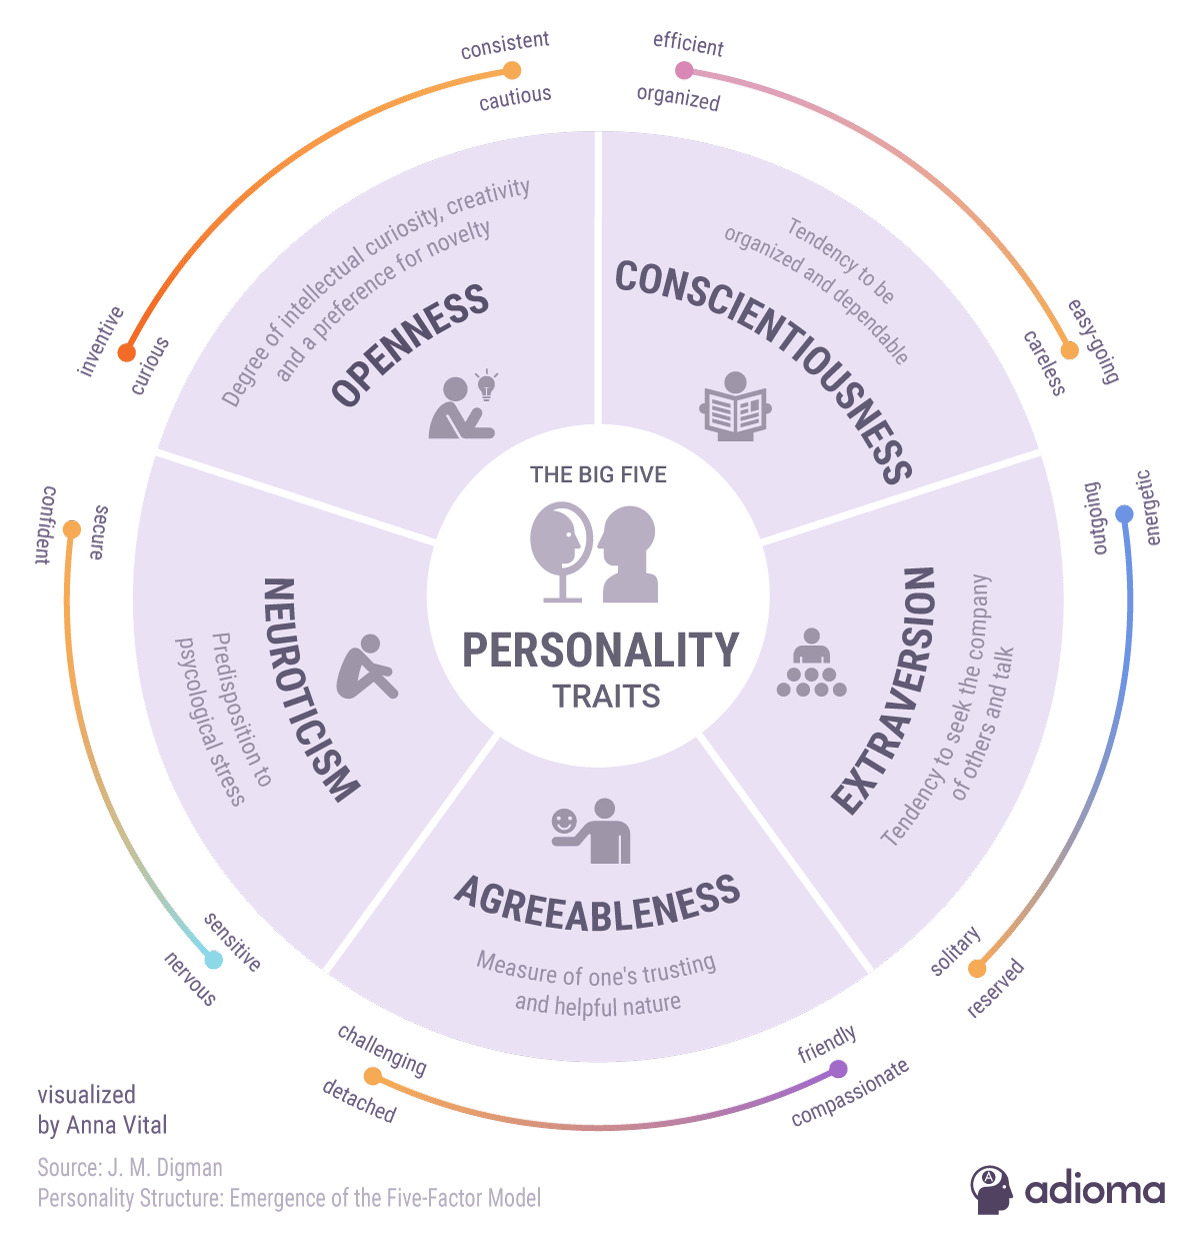
\includegraphics[height=.7\textheight]{pictures/traits2.jpeg}}
			\end{tabular}
		\end{tabular}
		
		
		
		%\begin{itemize}
		%	\item Openness
		%	\item Conscientiousness
		%	\item Extroversion
		%	\item Agreeableness
		%	\item Neuroticism
		%\end{itemize}
		%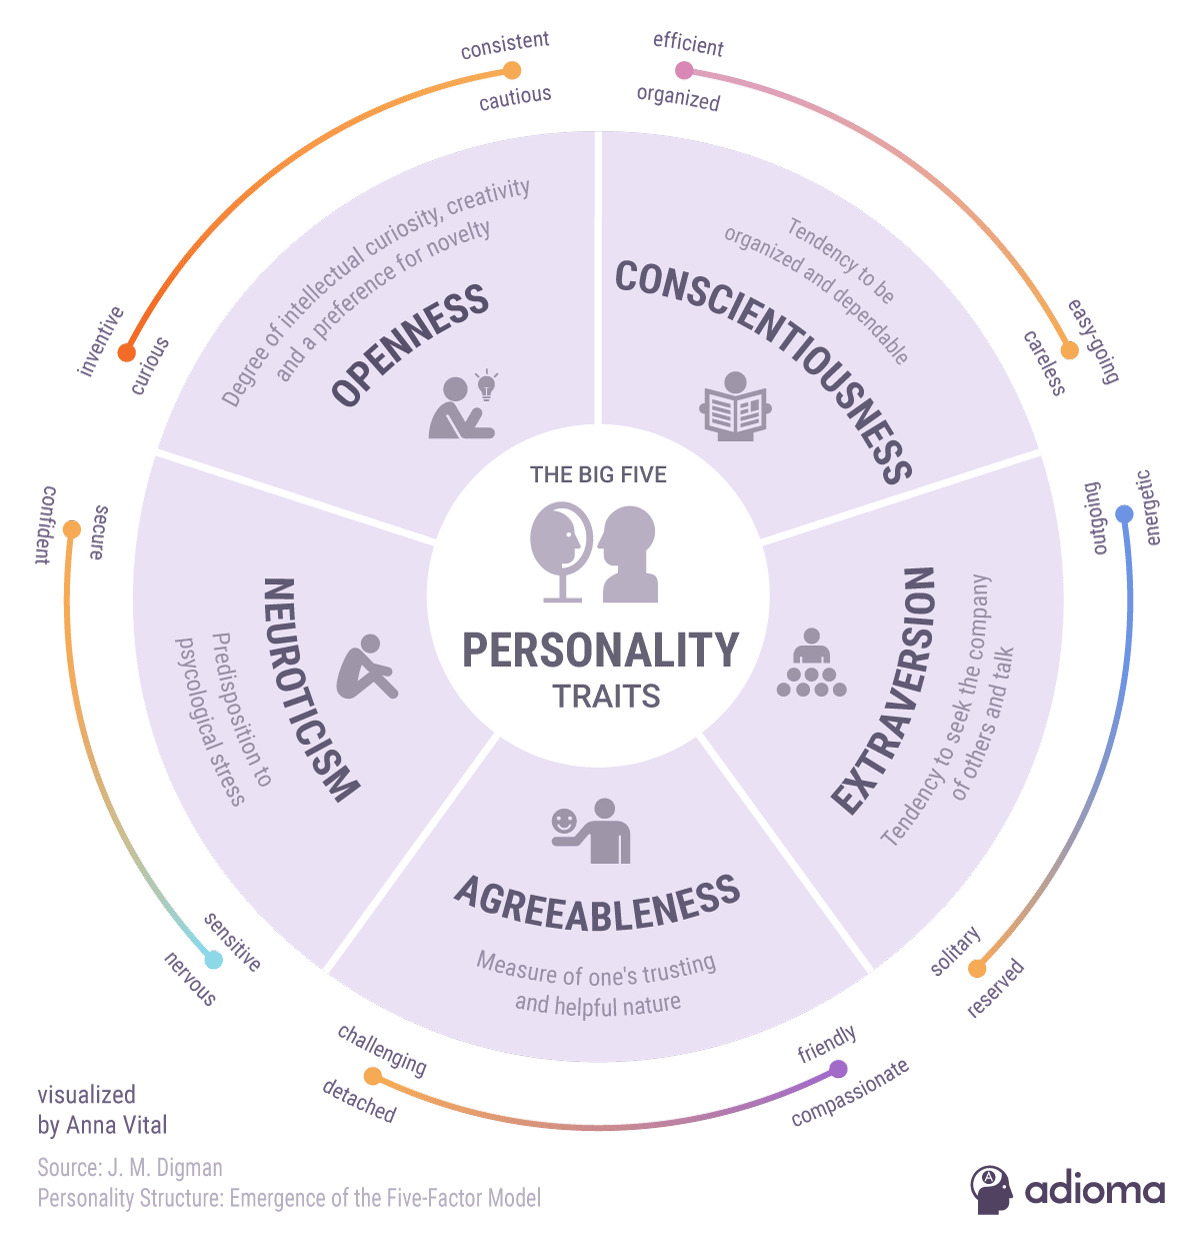
\includegraphics[height=.8\textheight, right]{pictures/traits2.jpeg}
	\end{frame}

	\begin{frame}
		\frametitle{What next?}
		Todo:
		\begin{itemize}
			\item Link the crawly output with the personality trait classifier.
			\item Program that takes data of a user and outputs the respective personality trait.
			\item Personality trait classifier using keywords and semantic similarity, compare results.
		\end{itemize}
	
		Sharing the work
		\begin{itemize}
			\item divide all tasks evenly
			\item still collaborate and help each other
		\end{itemize}
	\end{frame}
	
\end{document}